\chapter{CONCEITO DO SISTEMA}
\label{chap:conce}
A norma técnica (ISO-8373, 2012) criada para padronizar o vocabulário referente aos
robôs e dispositivos robóticos operando em ambientes industriais e não industriais, define o manipulador como uma máquina na qual o mecanismo, geralmente, consiste em uma série de segmentos, articulados ou deslizantes entre si, com o objetivo de empunhar e/ou mover objetos (peças ou ferramentas) em vários graus de liberdade. Em outras palavras, um manipulador é um equipamento programável baseado em atuadores, com um certo grau de liberdade, projetado para realizar uma variedade de atividades, assim como realização de diversos processos industriais \cite{ISO8373}.

Neste capítulo serão tratados os requisitos solicitados pelo cliente, os requisitos técnicos do projeto, o estudo do estado da arte sobre manipuladores e o ambiente de operação em que este manipulador realizará a atividade.

%------------------------------------------------------------------
\section{Parâmetros básicos}
\label{sec:basi}
Nesta seção encontram-se os requisitos solicitados pelo cliente, ou seja, a tarefa que precisa ser realizada e em qual ambiente o manipulador será simulado e concebido. Além disso, são exibidos os requisitos técnicos que tratam das especificações do sistema e uma breve revisão teórica de conceitos relacionados ao manipulador.

\subsection{Requisitos do cliente}
\label{sub:reqc}
Requisitos predeterminados pelo cliente consistem em exigências de funcionamento que devem ser observadas ao final do projeto, para que se considere um sucesso a concepção deste. Para tal, foram determinadas algumas característica desejáveis no projeto:
\begin{enumerate}
    \item Desenvolver um manipulador robótico.
    \item Realizar a tarefa de detecção de um marcador visual e acionamento do painel elétrico na orientação vertical e horizontal.
    \item Realizar a simulação do manipulador no ambiente \textit{\acs{ROS}} utilizando o software \textit{Gazebo}.
    \item Utilizar o \textit{framework} \textit{MoveIt} para o controle do  manipulador. 
    \item Realizar estudo estatístico para verificação da performance do manipulador.    
\end{enumerate}

\subsection{Requisitos técnicos}
\label{sub:reqt}
Os requisitos técnicos de um projeto são especificações necessárias para o funcionamento esperado do projeto. Podem ser sobrepostos aos requisitos do cliente em caso de conflito entre o esperado pelo cliente e o necessário para que o projeto seja bem sucedido, objetivando manter o projeto o mais eficiente dentro do escopo planejado. Os requisitos foram:
\begin{enumerate}
    \item O manipulador deve estar acoplado em uma base fixa situada a 0,28 m de uma das extremidades da bancada e centralizada com a mesma.
    \item Utilizar servo motores Dynamixel PH54-200-S500-R, PH54-100-S500-R e PH42-020-S300-R da Robotis. 
    \item Conter uma câmera RGB Teledyne Dalsa Genie Nano C2590. 
    \item Deverá possuir 5 graus de liberdade.
    \item Suportar uma carga máxima de 2 kg. 
    \item Ser capaz de acionar um painel elétrico.
    %\item Detecção de uma  \textit{tag} fixada a um painel elétrico. 
\end{enumerate}

\subsection{Estudo do estado da arte}
\label{sub:sota}

\par Com o advento do exponencial crescimento da tecnologia há um foco crescente na pesquisa e comercialização de robôs \cite{hernandez2018education}. Estes, por sua vez, são classificados em três grupos: manipuladores, veículos auto-guiados (\textit{\acs{AGV}}) e robôs móveis. Neste projeto, o objeto de interesse são os manipuladores robóticos, sistemas que possuem estrutura física similar a um braço humano. Estes robôs são compostos por partes rígidas, denominado de elos, conectados entre si por juntas \cite{santos2004robotica}. Esta estrutura encontra-se descrita na Figura \ref{fig:manipulador}.

\begin{figure}
    \caption{Elos e junta de um manipulador robótico.}
    \centering
    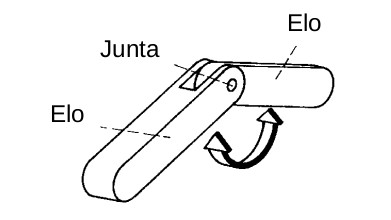
\includegraphics[scale=0.6]{images/manipulador.jpg}
    \legend{Fonte: \cite{santos2004robotica}.}
    \label{fig:manipulador}
\end{figure}

\par Muitas pesquisas vêm sido realizadas na área de manipuladores robóticos. Em \cite{hernandez2017design} é descrito o desenvolvimento de um manipulador robótico com 3 \textit{\acs{DoF}} e dois dedos independentes. Este robô foi desenvolvido com o propósito de manipular objetos, cujas localizações são conhecidas, e transportá-los de uma localidade para outra utilizando \textit{\acs{ROS}}. Os autores utilizaram o \textit{MoveIt} para tratar do planejamento de trajetória e o \textit{Rviz} como ferramenta de visualização. Além disso, foi desenvolvido um controlador de posição e força para o \textit{endeffector}\footnote{Na robótica, um endeffector é o dispositivo no final de um braço robótico, projetado para interagir com o meio ambiente.} durante o processo de \textit{pick and place}\footnote{Sequência de movimentos na qual o manipulador robótico pega determinado objeto e o transfere a uma pose alvo.}. Os experimentos realizados trouxeram bons resultados para o que foi proposto, sendo ressaltada a necessidade de adicionar um sistema de visão que permita identificar e localizar o objeto alvo. 

O planejamento de trajetória para um manipulador de 5 \textit{\acs{DoF}} a partir do \textit{MoveIt} é exibido em \cite{zhang2019motion}. A partir de um  modelo \textit{\acs{CAD}} já existente foi construído o modelo \textit{\acs{URDF}} utilizado para simulação no \textit{\acs{ROS}}. O processo de planejamento foi visualizado a partir do \textit{Rviz} e o caminho planejado foi transmitido para os servo-motores possibilitando ao manipulador executar a sua rotina. O robô tem como tarefa manipular um objeto alvo de um local para outro, identificado a partir de técnicas de visão computacional que combinam os algoritmos \textit{SIFT} e \textit{RANSAC}. OS resultados experimentais mostraram que o uso do \textit{MoveIt} reduz as dificuldades de operação para manipuladores e oferece vantagens em termos de validação de algoritmos e exploração de funções, sendo possível utilizar o método proposto para o controle em tempo real do robô. 

\par A aplicação de técnicas de visão computacional em um manipulador do tipo \textit{Robai Cyton Gamma 3000} é exibida em \cite{khan2018ros}. O robô é conectado com uma câmera externa via \textit{\acs{ROS}}, possui um \textit{endeffector} em forma de garra que segura uma estrutura similar a um prato, e tem como tarefa equilibrar uma bola localizada no centro do prato. Para realizar o controle da tarefa de equilíbrio, a bola é identificada a partir de um algoritmo escrito em C++ e que utiliza bibliotecas do \textit{\acs{OpenCV}}. As juntas do manipulador são atuadas a partir de servo-motores \textit{Dynamixel} que são diretamente controlados por um algoritmo. O sistema foi desenvolvido de forma que os componentes se comunicassem entre si para receber respostas do sistema de visão e dos motores, computá-las e enviar comandos de controle que permitissem executar a tarefa. Foram realizados testes e os resultados experimentais foram satisfatórios, sendo o manipulador capaz de equilibrar a bola em uma pequena vizinhança do centro do prato.

O uso de marcadores visuais do tipo \textit{ArUco} associados ao planejamento de trajetória para um manipulador robótico é abordado em \cite{javeed2019autonomous}. O manipulador encontra-se acoplado a uma plataforma móvel e tem como objetivo o transporte de objetos de forma autônoma em um determinado espaço. Os autores também descrevem a integração dos mecanismos de detecção do marcador visual, navegação do robô e planejamento de trajetória, realizados no \textit{\acs{ROS}}. O robô é capaz de estimar a pose do marcador, aproximar-se e realizar sua tarefa. Os testes realizandos mostraram a eficiência do sistema, sendo apontada a necessidade de um estudo futuro para possibilitar o planejamento de trajetória em um ambiente com obstáculos.
% \par Para que um manipulador possa se movimentar em um ambiente e realizar as tarefas propostas é necessário que sejam conhecidos sua orientação e posição em relação ao sistema de origem. Este conjunto de informações é denomidado de frame do robô e esta descrição constitui o sistema de referência de um manipulador robótico. Há sistemas transladados: onde a origem de um sistema está transladada em relação ao do manipulador; sistemas rotacionados: as origens do sistema de referência coincidem, porém um dos sistemas tem um dos eixos rotacionados em um ângulo $\alpha$ em relação ao outro; e há o sistema genérico, neste sabe-se a descrição de um vetor em relação a um sistema de referência. 

% Uma das primeiras 
% Para realizar o mapeamento genérico, cinemática direta, utiliza-se a Equação \ref{map_generico} onde $_{ }^{A}\textrm{P}$ é o vetor de posição no sistema de referência {A} descrevendo os pontos x, y e z deste sistema. Através da matriz de transformação homogênea, ${_{B}^{A}\textrm{T}}$ é possível realizar o mapeamento do manipulador em um sistema de referência em relação a outro, neste caso de {B} em relação a {A}. Esta matriz de transformação homogênea engloba as matrizes de rotação do sistema B em relação a A, ${_{B}^{A}\textrm{R}}$, e do vetor posição que localiza a origem do sistema de B $_{ }^{A}\textrm{P}_{BORG}$ \cite{mckerrow1991introduction}. 

% \begin{equation}
%     \label{map_generico}
%     _{ }^{A}\textrm{P} = {_{B}^{A}\textrm{T}} {_{ }^{B}\textrm{P}}    
% \end{equation}


% \par O estudo da dinâmica e da cinemática apresenta a síntese do projeto de um dispositivo, expressando matematicamente as relações de movimento de um mecanismo na execução de determinada tarefa.

% \par Após as configurações do sistema é necessário encontrar as equações de dinâmicas de movimento que podem ser obtidas pelo método de equações de movimento de Newton ou utilizando o cálculo variacional (Princípio de Hamilton ou Princípio da Mínima Ação) \cite{lima2017dinamica}.

% \par Para a análise cinemática, utiliza-se os parâmetros de Denavitt-Hartenberg (D-H). Este realiza uma cadeia cinemática espacial através da fixação de sistemas de referência aos elos \cite{paul1981robot}.  Esta notação de Denavit-Hartenberg é uma ferramenta comumente utilizada para sistematizar a descrição cinemática de sistemas mecânicos articulados com $\textit{n}$
% graus de liberdade \cite{uicker1964iterative}. Na Tabela \ref{tab:dh_table} tem-se a cadeia cinemática através dos parâmetros D-H para o manipulador da Figura \ref{fig:cinematica}, nesta tabela tem-se o elo (\textit{link}), $\theta$ refere-se ao ângulo de rotação no eixo z e $\alpha$ rotação no eixo x, \textit{a} refere-se a translação ao longo do eixo de rotação x e \textit{d} translação ao longo do eixo z. Na cinemática direta é possível observar que a partir dos ângulos das juntas do manipulador encontra-se a posição e orientação da ferramenta com relação a estação de trabalho. Contudo, quando projeta-se um manipulador, é fundamental realizar os cálculos da cinemática inversa. Nesta, por sua vez, são obtidos dados de posição e orientação da ferramenta com relação a estação de trabalho e calcula-se os ângulos das juntas \cite{craig2012robotica}.

% \par Para encontrar os ângulos de juntas necessários para posiocionar o sistema de referência da ferramenta (\textit{tool frame}) com relação ao sistema da estação de trabalho (\textit{station frame}), divide-se em duas partes. Primeiro, fazemos as transformações para encontrar o sistema do punho (\textit{wrist frame}) com relação ao sistema da base (\textit{base frame}) e depois usa-se a cinemática inversa para calcular os ângulos das juntas. O cálculo desses ângulos possibilita a construção de sistemas de controle que tradicionalmente utilizam matrizes jacobianas em conjunto com as pseudo-inversas \cite{wunderlich2004simulating}.

% \par  As soluções mais utilizadas para calcular a cinemática inversa são os métodos analíticos e numéricos iterativos. A escolha de um método depende de sua aplicação, do tipo de junta, da estrutura utilizada e da quantidade de graus de liberdade. Na maioria dos casos o método numérico é preferível quando se tem acesso ao um processamento computacional adequado. Existem diversos métodos numéricos iterativos, exemplo: O Newton-Raphson, algoritmo de Levenberg–Marquardt, o Jacobiano Pseudo-Inverso \cite{pinheiro2013cinematica}.




% \begin{figure}
%     \caption{Frames para o manipulador Elbow.}
%     \centering
%     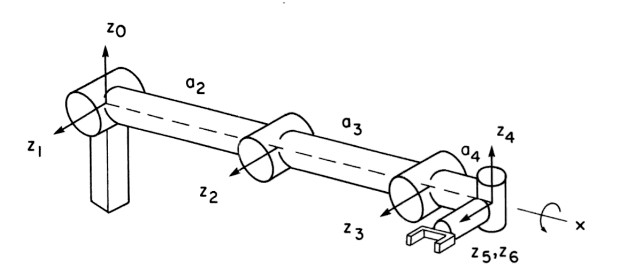
\includegraphics[scale=0.6]{images/cinematica.jpg}
%     \legend{Fonte: \cite{paul1981robot}.}    
%     \label{fig:cinematica}
% \end{figure}


% \begin{table}[H]
%     \caption{Parâmetros dos links para o manipulador Elbow.}
%     \centering
%     \begin{tabular}{|c|c|c|c|c|c|c|}
%     \hline
%     \textbf{Link} & \textbf{Variável}     & \textbf{$\alpha$} & \textbf{a} & \textbf{d} & \textbf{$\cos{\alpha}$} & \textbf{$\sin{\alpha}$} \\ \hline
%         1             & $\theta_{1}$ & 90º                            & 0          & 0          & 0                                  & 1                                   \\ \hline
%         2             & $\theta_{2}$                      & 0º                             & $a_{2}$         & 0          & 1                                  & 0                                   \\ \hline
%         3             & $\theta_{3}$                      & 0º                             & $a_{3}$         & 0          & 1                                  & 0                                   \\ \hline
%         4             & $\theta_{4}$                      & -90º                           & $a_{4}$         & 0          & 0                                  & -1                                  \\ \hline
%         5             & $\theta_{5}$                      & 90º                            & 0          & 0          & 0                                  & 1                                   \\ \hline
%         6             & $\theta_{6}$                      & 0º                             & 0          & 0          & 1                                  & 0                                   \\ \hline
%     \end{tabular}
%     \legend{Fonte: \cite{paul1981robot}.}
%     \label{tab:dh_table}
% \end{table}


% O controle da cinemática e o planejamento da movimentação evitam que o manipulador colida com outros elementos do seu espaço de trabalho. Para tal é necessário aplicar técnicas de controle e utilização de sensores, estes últimos fazem com que o robô tenha capacidade de percepção coletando dados tanto internos, sobre seu sistema mecânico, quanto externos, no meio ambiente em qual está inserido \cite{sciavicco2012modelling}.

% A dinâmica do manipulador dependerá do seu design mecânico, logo esta definição irá variar de um manipulador para outro, e depende também de já haver definido as formulações cinemáticas \cite{norton2001mecanismos}. Estas por sua vez, fornecem os elementos geométricos de um sistema que são a base para se obter as energias que compõem as equações dinâmicas.

% 
% \subsection{Características do manipulador}
% \label{sub:carac}
% Na Tabela \ref{tab:dh} encontra-se os parâmetros relacionados aos elos do manipulador Timon-HM descrito conforme a Figura \ref{fig:dh_config}.
% //todo uma subsection só para apresentar uma tabela?? porque? não faz sentido

% \begin{figure}[H]
%     \caption{Configuração D-H do manipulador Timon-HM.}
%     \centering
%     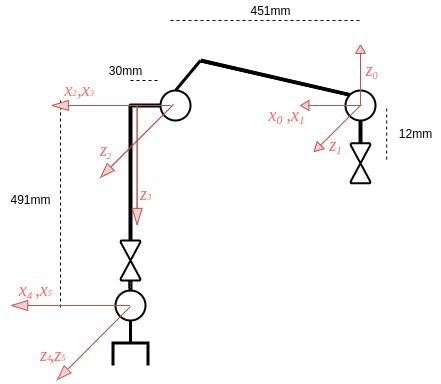
\includegraphics[scale=0.8]{images/dh_configuration.png}
%     \legend{Fonte: Autoria própria.}
%     \label{fig:dh_config}
% \end{figure}

% \begin{table}[H]
%     \caption{Parâmetros D-H para o manipulador Timon-HM.}
%     \centering
%     \begin{adjustbox}{max width=\textwidth}
%     \begin{tabular}{|c|c|c|c|c|}
%     \hline
%     \rowcolor[HTML]{EFEFEF} 
%     Link & a (mm) & $\alpha $(rad) & d (mm) & $\theta $(rad) \\ \hline
%     1 & 0   & $\pi / 2$ & 12  & 0                     \\ \hline
%     \rowcolor[HTML]{EFEFEF} 
%     2 & 452 & 0         & 0   & $\pi/2 - \arctan(30/451)$ \\ \hline
%     3 & 30  & $-\pi/2$  & 0   & $\pi/4 + \arctan(30/451)$ \\ \hline
%     \rowcolor[HTML]{EFEFEF} 
%     4 & 0   & $\pi/2$   & 491 & 0                     \\ \hline
%     5 & 0   & 0         & 0   & 0                     \\ \hline
%     \end{tabular}
%     \end{adjustbox}
%     \legend{Fonte: Autoria própria.}
%     \label{tab:dh}
%     \end{table}



% \subsection{Ambiente de operação}
% \label{sub:ambiente}
% //TODO lembrem-se não é caixa, é um painel elétrico:
% //TODO Jess corrigido
% O ambiente para a realização do desafio, onde serão incluídos o manipulador e um painel elétrico, é sobre uma mesa com 1.7 m de comprimento por 0.8 m de largura. Na Figura \ref{fig:simulacao} tem-se o ambiente de operação simulado no Gazebo para que possam ser realizados testes e para validação dos parâmetros aplicados ao manipulador.

% \par Nas Figuras \ref{fig:workspace_xy}, \ref{fig:workspace_xz} e \ref{fig:workspace_yz} estão descritos o \textit{workspace}, ambiente de operação do manipulador com as vistas dos eixos X-Y, X-Z e Y-Z, respectivamente. 
% A região em azul indica onde o manipulador consegue operar e a partir destas imagens é possível observar que o manipulador possui restrições de operação. Isso é devido às limitações existentes em cada junta.

% \begin{figure}[H]
%     \caption{Simulação no Gazebo}
%     \centering
%     \includegraphics[scale=0.34]{images/desafio.png}
%     \legend{Fonte: Autoria própria.}
%     \label{fig:simulacao}
% \end{figure}


% \begin{figure}[H]
%     \caption{Workspace do manipulador nos eixos X-Y.}
%     \centering
%     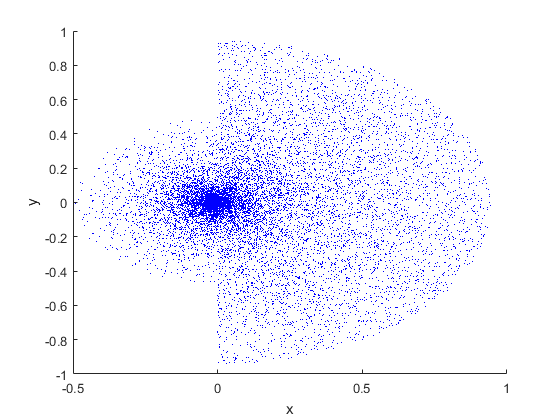
\includegraphics[scale=0.8]{images/workspace_xy.png}
%     \legend{Fonte: Autoria própria.}
%     \label{fig:workspace_xy}
% \end{figure}



% \begin{figure}[H]
%     \caption{Workspace do manipulador nos eixos X-Z.}
%     \centering
%     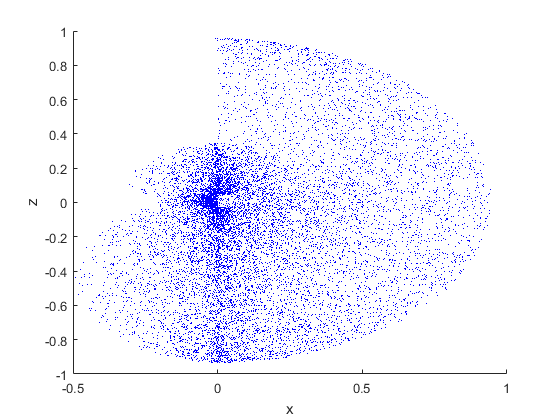
\includegraphics[scale=0.8]{images/workspace_xz.png}
%     \legend{Fonte: Autoria própria.}
%     \label{fig:workspace_xz}
% \end{figure}


% \begin{figure}[H]
%     \caption{Workspace do manipulador nos eixos Y-Z.}
%     \centering
%     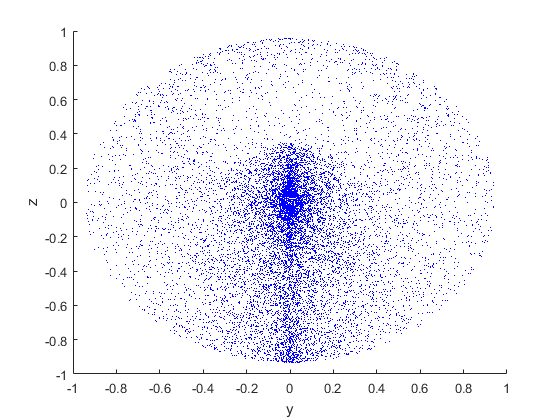
\includegraphics[scale=0.8]{images/workspace_yz.png}
%     \legend{Fonte: Autoria própria.}
%     \label{fig:workspace_yz}
% \end{figure}


%\subsection{Normas utilizadas}
%\label{sub:normas}

%EXTRA
%\subsection{Benchmarking}
%\label{sub:bench}

%EXTRA
%\subsection{Desdobramento da Função Qualidade}
%\label{sub:qfd}

%EXTRA
%\subsection{Matriz morfológica}
%\label{sub:matmorf}


